In this chapter a small we show how a Modelica model is compiled, translated and export to ProMoVis through the export tool. The files used are available throught the source code\cite{githabb}\nocite{*}.

\section{The input model}

If we take the following Modelica model: 
\lstset{language=modelica}
\begin{lstlisting}
package QuadTankPack
  model QuadTank
    // Process parameters
	parameter Modelica.SIunits.Area A1=4.9e-4, 
									A2=4.9e-4, 
									A3=4.9e-4, 
									A4=4.9e-4;
	parameter Modelica.SIunits.Area a1(min=1e-6)=0.03e-4, 
									a2=0.03e-4, 
									a3=0.03e-4, 
									a4=0.03e-4;
	parameter Modelica.SIunits.Acceleration g=9.81;
	
	parameter Real 	k1_nmp(unit="m^3/s/V") = 0.56e-6, 
					k2_nmp(unit="m^3/s/V") = 0.56e-6;
	parameter Real g1_nmp=0.30, g2_nmp=0.30;

    // Initial tank levels
	parameter Modelica.SIunits.Length x1_pmv_0 = 0.04102638;
	parameter Modelica.SIunits.Length x2_0 = 0.06607553;
	parameter Modelica.SIunits.Length x3_0 = 0.00393984;
	parameter Modelica.SIunits.Length x4_foo_0 = 0.00556818;
	
    // Tank levels
	Modelica.SIunits.Length x1_pmv(start=x1_pmv_0,min=0.0001);
	Modelica.SIunits.Length x2(start=x2_0,min=0.0001);
	Modelica.SIunits.Length x3(start=x3_0,min=0.0001);
	Modelica.SIunits.Length x4_foo(start=x4_foo_0,min=0.0001);
	Real x1plusx2(start=0);
	// Inputs
	input Modelica.SIunits.Voltage u1;
	input Modelica.SIunits.Voltage u2;

  equation    
    der(x1_pmv) = 	-a1/A1*sqrt(2*g*x1_pmv) + a3/A1*sqrt(2*g*x3) 
					+ g1_nmp*k1_nmp/A1*u1;						
	der(x2) 	= 	-a2/A2*sqrt(2*g*x2) + a4/A2*sqrt(2*g*x4_foo)
					+ g2_nmp*k2_nmp/A2*u2;
	x1plusx2	=	x2+x1_pmv;
	der(x3) 	= 	-a3/A3*sqrt(2*g*x3) 
					+ (1-g2_nmp)*k2_nmp/A3*u2;
	der(x4_foo) = 	-a4/A4*sqrt(2*g*x4_foo) 
					+ (1-g1_nmp)*k1_nmp/A4*u1;

  end QuadTank;
end QuadTankPack;
\end{lstlisting}
This is basically the same model as provided in the JModelica examples, the initial values of the states are just set so that the model is in equilibrium at time 0. There is also the addition of the variable, x1plusx2, just to make the example complete with both states and algebraic variables. 
\section{Running the export}
If we set up our xml file as depicted in chapter 3, and indicate that we want variables with "\_pmv", "foo\_" and "x2" to be measured variables in the resulting ProMoVis-representation. We then get the following SFG in ProMoVis:

\setlength\fboxsep{0pt}
\setlength\fboxrule{0.5pt}
\fbox{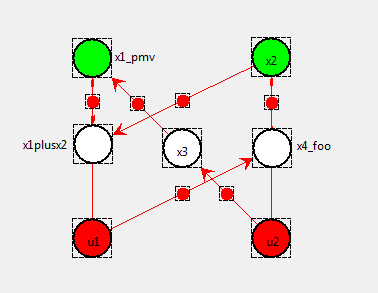
\includegraphics{Figures/exportSFG.png}}\\\newline
Here we see that x1\_pmv and x2 has been set as measured variables. None of the variable ended with foo\_.
What if we examine the extracted relations, if we first look at the x1plusx2 variable:\\\newline
\setlength\fboxsep{0pt}
\setlength\fboxrule{0.5pt}
\fbox{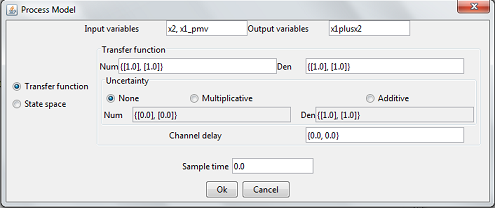
\includegraphics{Figures/x1plusx2Rel.png}}\\\newline
Here, due to the fact that we have represented all the variables as Multiple input, single output process models, it doesnt matter wich of the incoming arrows to z1plusx2 we examine, we will still see all of the inputs as depicted in the dialog. And as we can see, the transfer functions is just unity, for both of the input variables. \\\newline
\setlength\fboxsep{0pt}
\setlength\fboxrule{0.5pt}
\fbox{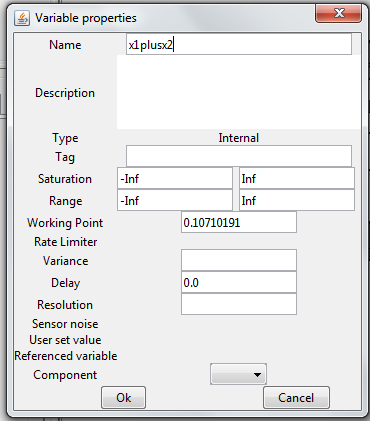
\includegraphics{Figures/x1plusx2OPP.png}}\\\newline
Naturally, since we have set the initial values for x1\_pmv and x2 ourselves, the operating point of x1plusx2 is the sum of the initial values.

